\subsection{Dynamic Models}\label{S02-2}

\begin{itemize}
\item[•] $\mathbb{\Re}$ Modelo do mecanismo \underline{R}\underline{R}

\begin{figure}[h!]
	\centering
	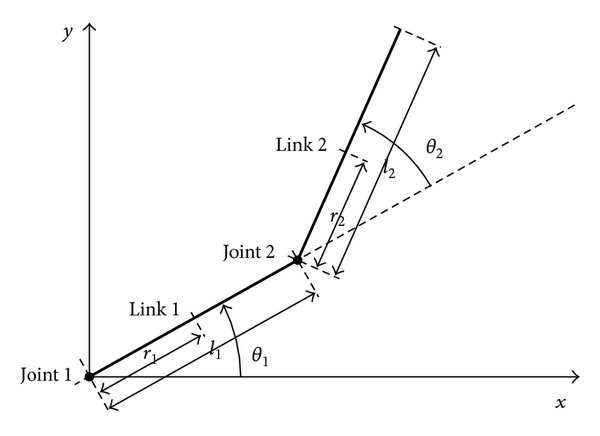
\includegraphics[scale=1.5]{RR.jpg}  
	\caption{Rob\^o \underline{R}\underline{R}}
	\label{fig:figura2}
\end{figure}

	\begin{itemize}
	\item[i)] Primeiro definimos $\nu_q$ coordenadas  $\mq$. Estas podem ser subdivididas em $\nu\ssh$ coordenadas independentes $\mq\ssh$ e $\nu_q^\circ$ 	coordenadas redudantes $\mq^\circ$.
	
	$$
	\mq = \begin{bmatrix}
	\mq\ssh \\
	\mq^\circ
	\end{bmatrix}
	$$

	No caso do mecanismo $\underline{R}\underline{R}$, temos:

	\begin{equation}
	\mq\ssh = \begin{bmatrix}
	\theta_1 & \theta_2
	\end{bmatrix}^T \\
	\end{equation}
	
	\begin{equation}
	\mq^\circ = \begin{bmatrix}
	x_1 & y_1 & x_2 & y_2
	\end{bmatrix}^T
	\end{equation}

	Com $\nu\ssh = 2$ e $\nu_q^\circ = 4$. Neste caso, as componentes de $\mq^\circ$ s\~ao as coordenadas dos centros de massa das barras, escritas no referencial 	inercial $O_{xy}$. \\
	
	\item[ii)] Depois definimos os vetores de velocidades absolutas:
	
	$$ \mw =
	\begin{bmatrix}
	\mw_\omega \\
	\mw_v
	\end{bmatrix}
	$$
	
	\begin{equation}
	\mw_\omega = \begin{bmatrix}
	\omega_{z_1} & \omega_{z_2}
	\end{bmatrix}^T
	\end{equation}
	
	\begin{equation}
	\mw_v = \begin{bmatrix}
	v_{x_1} & v_{y_1} & v_{x_2} & v_{y_2}
	\end{bmatrix}^T
	\end{equation}
	
	Sendo $\mw_v$ as componentes das velocidades absolutas dos centros de massa das barras, escritas nas bases presas às barras, e $\mw_\omega$ as componentes das velocidades angulares absolutas, escritas nas bases presas às barras. \\
	
	\item[iii)] Definimos $\nu_p$ coordenadas  $\mp$. Estas podem ser subdivididas em $\nu\ssh$ coordenadas independentes $\mp\ssh$ e $\nu_p^\circ$ coordenadas redudantes $\mp^\circ$. As coordenadas $\mp\ssh$ podem ser subdividas em $\nu_\omega\ssh$ velocidades angulares $\momega^{\#}$ e $\nu_v\ssh$ velocidades lineares $\mathbb{\nu}\ssh$. As coordenadas $\mp^\circ$ podem ser subdividas em $\nu_\omega^\circ$ velocidades angulares $\momega^\circ$ e $\nu_v^\circ$ velocidades lineares $\mathbb{\nu}^\circ$.
	
	
	\begin{multicols}{3}
	$ \mp = \begin{bmatrix}
	\mp\ssh \\
	\mp^\circ
	\end{bmatrix} $

	$ \mp\ssh = \begin{bmatrix}
	\momega\ssh \\
	\mathbb{\nu}\ssh
	\end{bmatrix} $

	$ \mp^\circ = \begin{bmatrix}
	\momega^\circ \\
	\mathbb{\nu}^\circ
	\end{bmatrix} $

	\end{multicols}
	
	Como \'e conveniente que as velocidades generalizadas $\mp$ sejam velocidades absolutas, escolhemos as componentes de $\mp$ como sendo as mesmas componentes de $\mw$, respeitando a ordena\c{c}\~ao indicada acima. \\ 

	No caso do mecanismo $\underline{R}\underline{R}$, temos:

	\begin{equation}
	\momega\ssh = \begin{bmatrix}
	\omega_{z_1} \\
	\omega_{z_2}
	\end{bmatrix}
	\end{equation}
	
	\begin{equation}
	\mathbb{\nu}\ssh = \emptyset
	\end{equation}		
	
	\begin{equation}
	\momega^\circ = \emptyset
	\end{equation}		
	
	\begin{equation}
	\mathbb{\nu}^\circ = \begin{bmatrix}
	v_{x_1} & v_{y_1} & v_{x_2} & v_{y_2}
	\end{bmatrix}^T
	\end{equation}\\

	Com $\nu_\omega\ssh = 2$, $\nu_v\ssh = 0$, $\nu_\omega^\circ = 0$, $\nu_v^\circ = 4$ e $\nu_p^\circ = \nu_\omega^\circ + \nu_v^\circ = 4$. \\
	
		\item[iv)] Realizamos a cinemática de posi\c{c}\~ao para os centros de massa das barras, de modo a relacionar as coordenadas $\mq^\circ$ com as coordenadas $\mq\ssh$. Para isso, utilizamos matrizes de transforma\c{c}\~ao homog\^enea.



	$$ \nmat{\vH}_{\ttB_0 \rl \ttB_1}  =
	\begin{bmatrix}
	 Rot(\theta_1, z_0) & \nmat{\overrightarrow{\ttO_0 \ttO_1}}_{\ttB_0} \\
	 \mzr_{2x1} & 1 \\
	\end{bmatrix}
	=
	\begin{bmatrix}
	 \ccos_1 & -\ssin_1 & 0 \\
	 \ssin_1 & \ccos_1 & 0 \\
	 0 & 0 & 1 \\
	\end{bmatrix} ;
	\begin{bmatrix}
	\nmat{\overrightarrow{\ttO_1 \ttG_1}}_{\ttB_1} \\
	1
	\end{bmatrix}
	=
	\begin{bmatrix}
	l_{1g} \\
	0 \\
	1 \\
	\end{bmatrix}
	$$

	$$ \nmat{\vH}_{\ttB_1 \rl \ttB_2} =
	\begin{bmatrix}
	 Rot(\theta_2, z_1) & \nmat{\overrightarrow{\ttO_1 \ttO_2}}_{\ttB_1} \\
	 \mzr_{2x1} & 1 \\
	\end{bmatrix}
	=
	\begin{bmatrix}
	 \ccos_2 & -\ssin_2 & l_1 \\
	 \ssin_2 & \ccos_2 & 0 \\
	 0 & 0 & 1 \\
	\end{bmatrix} ;
	\begin{bmatrix}
	 \nmat{\overrightarrow{\ttO_2 \ttG_2}}_{\ttB_2} \\
	1
	\end{bmatrix}
	=
	\begin{bmatrix}
	l_{2g} \\
	0 \\
	1 \\
	\end{bmatrix}
	$$

	$$
	\nmat{\vH}_{\ttB_0 \rl \ttB_2} = \nmat{\vH}_{\ttB_0 \rl \ttB_1} \nmat{\vH}_{\ttB_1 \rl \ttB_2}  =
	\begin{bmatrix}
	\ccos_{1+2} & -\ssin_{1+2} & l_1 \ccos_1 \\
	\ssin_{1+2} & \ccos_{1+2} & l_1 \ssin_1 \\
	0 & 0 & 1 \\
	\end{bmatrix}
	$$


	\begin{equation}
	\therefore \begin{bmatrix}
	x_1 \\
	y_1 \\
	1 \\
	\end{bmatrix}
	=
	\nmat{\vH}_{\ttB_0 \rl \ttB_1}
	\begin{bmatrix}
	\nmat{\overrightarrow{\ttO_1 \ttG_1}}_{\ttB_1} \\
	1
	\end{bmatrix}
	=
	\begin{bmatrix}
	 l_{1g} \ccos_1 \\
	 l_{1g} \ssin_1 \\
	 1 \\
	\end{bmatrix}
	\end{equation}

	\begin{equation}
	\begin{bmatrix}
	x_2 \\
	y_2 \\
	1 \\
	\end{bmatrix}
	=
	\nmat{\vH}_{\ttB_0 \rl \ttB_2}
	\begin{bmatrix}
	 \nmat{\overrightarrow{\ttO_2 \ttG_2}}_{\ttB_2} \\
	1
	\end{bmatrix}
	=
	\begin{bmatrix}
	 l_1 \ccos_1 + l_{2g} \ccos_{1+2} \\
	 l_1 \ssin_1 + l_{2g} \ssin_{1+2} \\
	 1 \\
	\end{bmatrix}
	\end{equation}

	Repare que a partir das matrizes de transforma\c{c}\~ao homogênea encontradas, encontramos também as seguintes matrizes de mudan\c{c}a de base:
	
	\begin{equation}
	\mR_1 = \nmat{\vone}_{\ttB_0 \rl \ttB_1} =
	\begin{bmatrix}
	 \ccos_1 & -\ssin_1  \\
	 \ssin_1 & \ccos_1  \\
	\end{bmatrix}
	\end{equation}
	
	\begin{equation}
	\mR_2 = \nmat{\vone}_{\ttB_0 \rl \ttB_2} =
	\begin{bmatrix}
	 \ccos_{1+2} & -\ssin_{1+2}  \\
	 \ssin_{1+2} & \ccos_{1+2}  \\
	\end{bmatrix}
	\end{equation}		

	Com a cinemática de posi\c{c}\~ao, conseguimos obter $\nu_q^\circ = 4$ equa\c{c}\~oes vinculares de posi\c{c}\~ao. Sendo assim, o vetor dos v\'inculos de posi\c{c}\~ao é dado por:
	
	
	\begin{equation}
	\mphi(\mq)
	=
	\begin{bmatrix}
	x_1 - l_{1g} \ccos_1 \\
	y_1 - l_{1g} \ssin_1 \\
	x_2 - l_1 \ccos_1 - l_{2g} \ccos_{1+2} \\
	y_2 - l_1 \ssin_1 - l_{2g} \ssin_{1+2} \\
	\end{bmatrix}
	\end{equation}
	
	\item[v)] Utilizamos as matrizes de rota\c{c}\~ao para calcular as velocidades angulares em fun\c{c}\~ao de $\mq\ssh$ e $\dot{\mq}\ssh$:
	
	\begin{equation}
	\nsmat{\vomega_1}_{\ttB_1 \rl \ttB_1}  = \mR_1^T \dot{\mR}_1 =
	\begin{bmatrix}
	0 & -\dot{\theta}_1  \\
	\dot{\theta}_1 & 0  \\
	\end{bmatrix}
	\Rightarrow
	\nmat{\vomega_1}_{\ttB_1} = \dot{\theta}_1 \hat{k}
	\end{equation}
	
	\begin{equation}
	\nsmat{\vomega_2}_{\ttB_2 \rl \ttB_2} = \mR_2^T \dot{\mR}_2 =
	\begin{bmatrix}
	0 & -\dot{\theta}_1 -\dot{\theta}_2 \\
	\dot{\theta}_1 + \dot{\theta}_2 & 0  \\
	\end{bmatrix}
	\Rightarrow
	\nmat{\vomega_2}_{\ttB_2} = (\dot{\theta}_1 + \dot{\theta}_2) \hat{k}
	\end{equation}
	
	\item[vi)] Derivamos as equa\c{c}\~oes de posi\c{c}\~ao ((29) e (30)) para encontrar as velocidades dos centros de massa:
	
	\begin{equation}
	\nmat{\vv_1}_{\ttB_0} =
	\begin{bmatrix}
	\dot{x}_1 \\
	\dot{y}_1 \\
	\end{bmatrix}
	=
	\begin{bmatrix}
	- l_{1g} \ssin_1 \dot{\theta}_1 \\
	l_{1g} \ccos_1 \dot{\theta}_1 \\
	\end{bmatrix}
	\end{equation}
	
	\begin{equation}
	\nmat{\vv_2}_{\ttB_0} =
	\begin{bmatrix}
	\dot{x}_2 \\
	\dot{y}_2 \\
	\end{bmatrix}
	=
	\begin{bmatrix}
	- l_1 \ssin_1 \dot{\theta}_1 - l_{2g} \ssin_{1+2} ( \dot{\theta}_1 + \dot{\theta}_2)  \\
	l_1 \ccos_1 \dot{\theta}_1 + l_{2g} \ccos_{1+2} ( \dot{\theta}_1 + \dot{\theta}_2)  \\
	\end{bmatrix}
	\end{equation}
	
	\item[vii)] Passamos as velocidades dos centros de massa para as bases presas nas barras:

	$$ \nmat{\vv_1}_{\ttB_1} = \nmat{\vone}_{\ttB_1 \rl \ttB_0} \nmat{\vv_1}_{\ttB_0} = \mR_1^T \nmat{\vv_1}_{\ttB_0} $$
	$$ \nmat{\vv_2}_{\ttB_2} = \nmat{\vone}_{\ttB_2 \rl \ttB_0} \nmat{\vv_2}_{\ttB_0} = \mR_2^T \nmat{\vv_2}_{\ttB_0} $$
	
	Definindo:
	
	
	\begin{equation}
	\mR_\Diamond =
	\begin{bmatrix}
	\mR_1 & \mzr_{2x2} \\
	\mzr_{2x2} & \mR_2
	\end{bmatrix}
	\end{equation}
	
	Temos:
	
	\begin{equation}
	\mw_v = \mR_\Diamond^T \dot{\mq}^\circ
	\end{equation}
	
	
	\begin{equation}
	\therefore
	\begin{bmatrix}
	v_{x_1} \\
	v_{y_1} \\
	v_{x_2} \\
	v_{y_2} \\
	\end{bmatrix}
	=
	\begin{bmatrix}
	\ccos_1 & -\ssin_1 & 0 & 0 \\
	\ssin_1 & \ccos_1 & 0 & 0 \\
	0 & 0 & \ccos_{1+2} & -\ssin_{1+2} \\
	0 & 0 & \ssin_{1+2} & \ccos_{1+2} \\
	\end{bmatrix}^T
	\begin{bmatrix}
	\dot{x}_1 \\
	\dot{y}_1 \\	
	\dot{x}_2 \\
	\dot{y}_2 \\	
	\end{bmatrix}
	=
	\begin{bmatrix}
	0 \\
	l_{1g} \dot{\theta}_1 \\
	l_1 \ssin_2 \dot{\theta}_1\\
	(l_1 \ccos_2 + l_{2g} )\dot{\theta}_1 + l_{2g} \dot{\theta}_2 \\
	\end{bmatrix}
	\end{equation}
	
	\item[viii)] Montamos os vetores $\mp\ssh$ e $\mp^\circ$ em fun\c{c}\~ao de $\mq\ssh$ e $\dot{\mq}\ssh$:

	\begin{equation}
	\mp\ssh = 
	\begin{bmatrix}
	\omega_{z_1} \\
	\omega_{z_2} \\
	\end{bmatrix}
	= \mp\ssh_\star (\mq\ssh, \dot{\mq}\ssh ) =
	\begin{bmatrix}
	\dot{\theta}_1 \\
	\dot{\theta}_1 +\dot{\theta}_2 \\
	\end{bmatrix}
	\end{equation}
	
	\begin{equation}
	\mp^\circ = 
	\begin{bmatrix}
	v_{x_1} \\
	v_{y_1} \\
	v_{x_2} \\
	v_{y_2} \\
	\end{bmatrix}
	= \mp^\circ_ \star (\mq\ssh, \dot{\mq}\ssh ) =
	\begin{bmatrix}
	0 \\
	l_{1g} \dot{\theta}_1 \\
	l_1 \ssin_2 \dot{\theta}_1\\
	(l_1 \ccos_2 + l_{2g} )\dot{\theta}_1 + l_{2g} \dot{\theta}_2 \\
	\end{bmatrix}
	\end{equation}
	
	\item[ix)] Utilizando o fato de que $\mp\ssh_\star (\mq\ssh, \dot{\mq}\ssh )$ e $\mp^\circ_ \star (\mq\ssh, \dot{\mq}\ssh )$ s\~ao lineares em $\dot{\mq}\ssh$, encontramos as transforma\c{c}\~oes lineares $\mathbb{\Psi}(\mq)$ e $\mathbb{\Upsilon}(\mq)$ e o vetor dos v\'inculos de velocidades $\mathbb{\Lambda}(\mq,\mp)$:
	
	\begin{equation}
	\mp\ssh = \mp\ssh_\star (\mq\ssh, \dot{\mq}\ssh ) = \frac{\partial \mp\ssh_\star}{\partial \dot{\mq}\ssh} \dot{\mq}\ssh = \mathbb{\Psi} \dot{\mq}\ssh
	\end{equation}
	
	\begin{equation}
	\mp^\circ = \mp^\circ_\star (\mq\ssh, \dot{\mq}\ssh ) = \frac{\partial \mp^\circ_\star}{\partial \dot{\mq}\ssh} \dot{\mq}\ssh = \mathbb{\Upsilon} \dot{\mq}\ssh
	\end{equation}

	No caso do mecanismo $\underline{R}\underline{R}$, temos:
	
	\begin{equation}
	\mathbb{\Psi} = \frac{\partial \mp\ssh_\star}{\partial \dot{\mq}\ssh} =
	\begin{bmatrix}
	1 & 0  \\
	1 & 1  \\
	\end{bmatrix}
	\end{equation}
	
	\begin{equation}
	\mathbb{\Upsilon} = \frac{\partial \mp^\circ_\star}{\partial \dot{\mq}\ssh} =
	\begin{bmatrix}
	0 & 0 \\
	l_{1g} & 0 \\
	l_1 \ssin_2 & 0 \\
	l_1 \ccos_2 + l_{2g} & l_{2g} 
	\end{bmatrix}
	\end{equation}\\

	Como $\mp\ssh$ e $\dot{\mq}\ssh$ s\~ao independentes e tem o mesmo tamanho:

	$$ \dot{\mq}\ssh = \mathbb{\Psi}^{-1} \mp\ssh $$
	$$ \Rightarrow  \mp^\circ = \mathbb{\Upsilon} \mathbb{\Psi}^{-1} \mp\ssh $$
	\begin{equation}
	\therefore \mathbb{\Lambda}(\mq,\mp) = \mathbb{\Upsilon} \mathbb{\Psi}^{-1} \mp\ssh - \mp^\circ  = 0
	\end{equation}
	
	\item[x)] A partir dos v\'inculos de velocidades, encontramos a matriz $\mathbb{C}$ dos v\'inculos cinem\'aticos:
	
	$$ \mp^\circ = \mathbb{\Upsilon} \mathbb{\Psi}^{-1} \mp\ssh \Rightarrow \mp =
	\begin{bmatrix}
	\mone\\
	\mathbb{\Upsilon} \mathbb{\Psi}^{-1}
	\end{bmatrix}
	\mp\ssh
	$$
	
	\begin{equation}
	\therefore \mathbb{C} =
	\begin{bmatrix}
	\mone\\
	\mathbb{\Upsilon} \mathbb{\Psi}^{-1}
	\end{bmatrix}
	=
	\begin{bmatrix}
	1 & 0 \\
	0 & 1 \\
	0 & 0 \\
	l_{1g} & 0\\
	l_1 s_{2} & 0 \\
	l_1 c_{2} & l_{2g} \\
	\end{bmatrix}
	\end{equation}
	
	\item[xi)] Como (39) e (43) s\~ao transforma\c{c}\~oes invers\'iveis, encontramos a transforma\c{c}\~ao linear $\mathbb{\Gamma}(\mq)$:
	
	\begin{equation}
	\dot{\mq} =
	\begin{bmatrix}
	\dot{\mq}^{\#} \\
	\dot{\mq}^\circ \\
	\end{bmatrix}
	= \dot{\mq}_\star(\mq,\mp) =
	\begin{bmatrix}
	\mathbb{\Psi}^{-1} (\mq) \mp\ssh \\
	\mR_\Diamond (\mq) \mw_v (\mp)
	\end{bmatrix}
	=
	\begin{bmatrix}
	\omega_{z_1} \\
	\omega_{z_2}-\omega_{z_1}\\
	v_{x_1} \, \ccos_1 - v_{y_1} \, \ssin_1 \\
	v_{x_1} \, \ssin_1 + v_{y_1} \, \ccos_1 \\
	v_{x_2} \, \ccos_{1+2} - v_{y_2} \, \ssin_{1+2} \\
	v_{x_2} \, \ssin_{1+2} + v_{y_2} \, \ccos_{1+2} \\
	\end{bmatrix}
	\end{equation}
	
	\begin{equation}
	\mathbb{\Gamma}(\mq) = \frac{\partial \dot{\mq}_\star}{\partial \mp} =
	\begin{bmatrix}
	1 & 0 & 0 & 0 & 0 & 0 \\
	-1 & 1 & 0 & 0 & 0 & 0 \\
	0 & 0 & \ccos_1 & -\ssin_1 & 0 & 0 \\
	0 & 0 & \ssin_1 & \ccos_1 & 0 & 0 \\
	0 & 0 & 0 & 0 & \ccos_{1+2} & -\ssin_{1+2} \\
	0 & 0 & 0 & 0 & \ssin_{1+2} & \ccos_{1+2} \\
	\end{bmatrix}
	\end{equation}

	\item[xii)] Aplicamos o métodos de Gibbs-Appel extendido: \\
	
	O método de Gibbs-Appell apresenta certa simularidade com o método de Lagrange, pois utiliza derivadas de uma fun\c{c}\~ao energia para encontrar a equa\c{c}\~oes de movimento do sistema. Por\'em, a fun\c{c}\~ao energia utilizada não é a energia cinética, mas sim a energia de acelera\c{c}\~oes. A energia de acelera\c{c}\~oes para um corpo r\'igido \'e dada pela seguinte express\~ao:

	$$ \mathcal{S} = \frac{1}{2} m ( \va_G \cdot \va_G ) + \frac{1}{2}( \dot{\vomega} \cdot \vI \dot{\vomega} + 2 \dot{\vomega} (\vomega \wedge 	\vI \vomega )  )  $$
 
	Sendo $m$ a massa do corpo r\'igido, $\vI$ seu tensor de in\'ercia, $\va_G$ o vetor acelera\c{c}\~ao absoluta de seu centro de massa e $\vomega$ o vetor velocidade angular absoluta.  \\

	O modelo dinâmico utilizando o método de Gibbs-Appel extendido, é dado pela seguinte expressão:
	
	\begin{equation}
	\mC(q)^T ( \mM(\mq) \dot{\mp} + \mv(\mq,\mp) + \mg(\mq)) = (\mathbb{\Psi}^T)^{-1} \mf_{\dot{\mq}\ssh} 
	\end{equation}
	
	Com:
	
	\begin{equation}
	\mM(\mq) = \frac{\partial^2 \mathcal{S}}{\partial \dot{\mp}^2}
	\end{equation}
	
	\begin{equation}
	\mv(\mq,\mp) =  \frac{\partial \mathcal{S}}{\partial \dot{\mp}} - \frac{\partial^2 \mathcal{S}}{\partial \dot{\mp}^2} \dot{\mp}
	\end{equation}
	
	\begin{equation}
	\mg(\mq) =  \mathbb{\Gamma}^T \frac{\partial E_p}{\partial \mq}
	\end{equation}
	
	Sendo $E_p$ a energia potencial do sistema e $\mf_{\dot{\mq}\ssh}$ os esfor\c{c}os nas dire\c{c}\~oes de $\dot{q}^{\#}$. \\
	
	Como j\'a calculamos os vetores de velocidades absolutas dos centros de massa e de velocidades angulares absolutas, escritos em bases presas às barras, as acelera\c{c}\~oes absolutas dos centros de massa são dadas por:
	
	$$ \nvct{\va_i}_{\ttB_i} = \frac{\dd}{\dd t} \nvct{ \vv_i }_{\ttB_i} + \nsmat{\vomega_i}_{\ttB_i \rl \ttB_i}  \nvct{ \vv_i }_{\ttB_i} $$
	
	Como o mecanismo é plano:
	
	$$\nvct{\va_i}_{\ttB_i} = 
	\begin{bmatrix}
	\dot{v}_{x_i} \\
	\dot{v}_{y_i} \\
	\end{bmatrix}
	+
	\begin{bmatrix}
	0  & -\omega_{z_i} \\
	\omega_{z_i} & 0 \\
	\end{bmatrix}
	\begin{bmatrix}
	v_{x_i} \\
	v_{y_i} \\
	\end{bmatrix}
	=
	\begin{bmatrix}
	\dot{v}_{x_i} - \omega_{z_i} v_{y_i} \\
	\dot{v}_{y_i} + \omega_{z_i} v_{x_i}
	\end{bmatrix}
	 $$
	
	No caso do mecanismo $\underline{R}\underline{R}$, temos:
	
	\begin{equation}
	\mathcal{S} = \frac{1}{2} \Big( m_1 ( (\dot{v}_{x_1} - \omega_{z_1} v_{y_1})^2 + (\dot{v}_{y_1} + \omega_{z_1} v_{x_1})^2 ) + m_2 ( (\dot{v}_{x_2} - \omega_{z_2} v_{y_2})^2 + (\dot{v}_{y_2} + \omega_{z_2} v_{x_2})^2  ) + J_{z_1} \dot{\omega}_{z_1}^2 + J_{z_2} \dot{\omega}_{z_2}^2 \Big)
	\end{equation}
	
	\begin{equation}
	E_p = m_1 g y_1 + m_2 g y_2
	\end{equation}
	
	Calculando as derivadas:
	
	\begin{equation}
	\mM(\mq) =
	\begin{bmatrix}
	J_{z_1} & 0 & 0 & 0 & 0 & 0 \\
	0 & J_{z_2} & 0 & 0 & 0 & 0 \\
	0 & 0 & m_1 & 0 & 0 & 0 \\
	0 & 0 & 0 & m_1 & 0 & 0 \\
	0 & 0 & 0 & 0 & m_2 & 0 \\
	0 & 0 & 0 & 0 & 0 & m_2 \\
	\end{bmatrix}
	\end{equation}
	
	\begin{equation}
	\mv(\mq,\mp) =
	\begin{bmatrix}
	0 \\
	0 \\
	-m_1 \omega_{z_1} v_{y_1} \\
	m_1 \omega_{z_1} v_{x_1} \\
	-m_2 \omega_{z_2} v_{y_2} \\
	m_2 \omega_{z_2} v_{x_2} \\
	\end{bmatrix}
	\end{equation}
	
	\begin{equation}
	\mg =
	g \begin{bmatrix}
	0 \\
	0 \\
	m_1  \ssin_1 \\
	m_1  \ccos_1 \\
	m_2  \ssin_{1+2} \\
	m_2  \ccos_{1+2}\\
	\end{bmatrix}
	\end{equation}
	
	Sendo assim, o modelo dinâmico para o mecanismo \underline{R}\underline{R} é dado por:
	
	\begin{equation}
	\begin{bmatrix}
	1 & 0 \\
	0 & 1 \\
	0 & 0 \\
	l_{1g} & 0\\
	l_1 \ssin_{2} & 0 \\
	l_1 \ccos_{2} & l_{2g} \\
	\end{bmatrix}^T
	\begin{Bmatrix}
		\begin{bmatrix}
		J_{z_1} \dot{\omega}_{z_1} \\
		J_{z_2} \dot{\omega}_{z_2} \\
		m_1 \dot{v}_{x_1} \\ 
		m_1 \dot{v}_{y_1} \\
		m_2 \dot{v}_{x_2} \\
		m_2 \dot{v}_{y_2} \\
		\end{bmatrix}
		+
		\begin{bmatrix}
		0 \\
		0 \\
		-m_1 \omega_{z_1} v_{y_1} \\
		m_1 \omega_{z_1} v_{x_1} \\
		-m_2 \omega_{z_2} v_{y_2} \\
		m_2 \omega_{z_2} v_{x_2} \\
		\end{bmatrix}
		+
		g \begin{bmatrix}
		0 \\
		0 \\
		m_1  \ssin_1 \\
		m_1  \ccos_1 \\
		m_1  \ssin_{1+2} \\
		m_1  \ccos_{1+2}\\
		\end{bmatrix}
	\end{Bmatrix}
	=
	\begin{bmatrix}
	1 & 1 \\
	0 & 1 \\
	\end{bmatrix}^{-1}
	\begin{bmatrix}
	\tau_{1} \\
	\tau_{2} \\
	\end{bmatrix}
	\end{equation}
	
	Repare que o modelo não depende das coordenadas $\mq^\circ$. Elas foram uteis para a dedu\c{c}\~ao do modelo, mas com o modelo deduzido elas não tem mais utilidade.
	
	
	
	
	\end{itemize}
\end{itemize}

\begin{itemize}

\item Massa pontual:

\begin{equation}
	\mq_n = \begin{bmatrix}
	x_n \\
	y_n \\
	\end{bmatrix}
	=
	\begin{bmatrix}
	q_{n,1} \\
	q_{n,2} \\
	\end{bmatrix}
\end{equation}

\begin{equation}
	\mp_n = \begin{bmatrix}
	p_{n,1} \\
	p_{n,2} \\
	\end{bmatrix}
	=
	\begin{bmatrix}
	1 & 0 \\
	0 & 1 \\
	\end{bmatrix}
	\begin{bmatrix}
	\dot{q}_{n,1} \\
	\dot{q}_{n,2} \\
	\end{bmatrix}
\end{equation}

\begin{equation}
	\begin{cases}

	\begin{bmatrix}
	\dot{q}_{n,1} \\
	\dot{q}_{n,2} \\
	\end{bmatrix}
	=
	\begin{bmatrix}
	1 & 0 \\
	0 & 1 \\
	\end{bmatrix}
	\begin{bmatrix}
	p_{n,1} \\
	p_{n,2} \\
	\end{bmatrix} \\

	\begin{bmatrix}
	M_n \dot{p}_{n,1} \\
	M_n \dot{p}_{n,2} \\
	\end{bmatrix}
	+
	g \begin{bmatrix}
	0 \\
	M_n \\
	\end{bmatrix}
	=
	\begin{bmatrix}
	f_{n, 1} \\
	f_{n, 2} \\
	\end{bmatrix}
	\end{cases}
\end{equation}

Que pode ser reescrito como:

$$
\begin{bmatrix}
M_n & 0 \\
0 & M_n \\
\end{bmatrix}
\begin{bmatrix}
\ddot{q}_{n,1} \\
\ddot{q}_{n,2} \\
\end{bmatrix}
+
g \begin{bmatrix}
0 \\
M_n \\
\end{bmatrix}
=
\begin{bmatrix}
f_{n,1} \\
f_{n,2} \\
\end{bmatrix}
$$

\item RR:

\begin{equation}
	\mq_n = \begin{bmatrix}
	\theta_{1 \, n} \\
	\theta_{2 \, n} \\
	\end{bmatrix}
	=
	\begin{bmatrix}
	q_{n,1} \\
	q_{n,2} \\
	\end{bmatrix}
\end{equation}

\begin{equation}
	\mp_n = \begin{bmatrix}
	p_{n,1} \\
	p_{n,2} \\
	p_{n,3} \\
	p_{n,4} \\
	p_{n,5} \\
	\end{bmatrix}
	=
	\begin{bmatrix}
	1 & 0 \\
	1 & 1 \\
	l_{g1} & 0\\
	l_1 \ssin_{n,2} & 0 \\
	l_{g2} + l_1 \ccos_{n,2} & l_{g2}
	\end{bmatrix}
	\begin{bmatrix}
	\dot{q}_{n,1} \\
	\dot{q}_{n,2} \\
	\end{bmatrix}
\end{equation}

\begin{equation}
	\begin{cases}

	\begin{bmatrix}
	\dot{q}_{n,1} \\
	\dot{q}_{n,2} \\
	\end{bmatrix}
	=
	\begin{bmatrix}
	1 & 0 \\
	-1 & 1\\
	\end{bmatrix}
	\begin{bmatrix}
	p_{n,1} \\
	p_{n,2} \\
	\end{bmatrix} \\


	\begin{bmatrix}
	1 & 0 \\
	1 & 1 \\
	\end{bmatrix}^T
	\begin{bmatrix}
	 1 & 0 \\
	 0 & 1 \\
	 l_{g1} & 0 \\
	 l_1 \ssin_{n,2} & 0 \\
	 l_1 \ccos_{n,2} & l_{g2} \\
	\end{bmatrix}^T
	\begin{Bmatrix}
		\begin{bmatrix}
		J_{z1} \dot{p}_{n,1} \\
		J_{z2} \dot{p}_{n,2} \\
		m_1 \dot{p}_{n,3} \\
		m_2 \dot{p}_{n,4} \\
		m_2 \dot{p}_{n,5} \\
		\end{bmatrix}
		+
		\begin{bmatrix}
		0 \\
		0 \\
		0 \\
		- m_1 p_{n,2} p_{n,5} \\
		  m_1 p_{n,2} p_{n,4} \\
		\end{bmatrix}
		+
		g \begin{bmatrix}
		0 \\
		0 \\
		m_1 \ccos_{n,1} \\
		m_2 \ssin_{n,1+2} \\
		m_2 \ccos_{n,1+2} \\
		\end{bmatrix}
	\end{Bmatrix}
	=
	\begin{bmatrix}
	u_{n,1} \\
	u_{n,2}
	\end{bmatrix} \\

	\begin{bmatrix}
	l_{g1} & 0 & -1 & 0 & 0 \\
	l_1 \ssin_{n,2} & 0 & 0 & -1 & 0 \\
	l_1 \ccos_{n,2} & l_{g2}  & 0 & 0 & -1 \\
	\end{bmatrix}
	\begin{bmatrix}
	\dot{p}_{n,1} \\
	\dot{p}_{n,2} \\
	\dot{p}_{n,3} \\
	\dot{p}_{n,4} \\
	\dot{p}_{n,5} \\
	\end{bmatrix}
	=
	-
	\begin{bmatrix}
	0 \\
	l_1 \ccos_{n,2} p_{n,1} (-p_{n,1}+p_{n,2}) \\
	l_1 \ssin_{n,2} p_{n,1} (p_{n,1}-p_{n,2}) \\
	\end{bmatrix}

	\end{cases}
\end{equation}

Que pode ser reescrito como:

$$
\begin{bmatrix}
J_{z1} + J_{z2} + m_1 l_{g1}^2 + m_2 (l_1^2 + 2 l_1 l_{g2} \ccos_{n,2} + l_{g2}^2) & J_{z2} + m_2 l_{g2} (l_1 \ccos_{n,2} + l_{g2}) \\
J_{z2} + m_2 l_{g2} (l_1 \ccos_{n,2} + l_{g2}) & J_{z2} + m_2 l_{g2}^2
\end{bmatrix}
\begin{bmatrix}
\ddot{q}_{n,1} \\
\ddot{q}_{n,2} \\
\end{bmatrix}
$$
$$
+
\begin{bmatrix}
- m_2 l_1 l_{g2} \ssin_{n,2} \dot{q}_{n,2}^2 -2 m_2 l_1 l_{g2} \ssin_{n,2} \dot{q}_{n,1}  \dot{q} _{n,2} \\
m_2 l_1 l_{g2} \ssin_{n,2} \dot{q}_{n,1}^2 \\
\end{bmatrix}
+
g \begin{bmatrix}
m_1 l_{g1} \ccos_{n,1} + m_2 (l_{g2} \ccos_{n,1+2} + l_1 \ccos_{n,1}) \\
 m_2 l_{g2} \ccos_{n,1+2} \\
\end{bmatrix}
=
\begin{bmatrix}
u_{n,1} \\
u_{n,2} \\
\end{bmatrix}
$$

\item RR (0) com 2 massas acopladas (1 e 2):

\begin{equation}
	\begin{cases}

	\begin{bmatrix}
	\dot{q}_{0,1} \\
	\dot{q}_{0,2} \\
	\end{bmatrix}
	=
	\begin{bmatrix}
	1 & 0 \\
	-1 & 1\\
	\end{bmatrix}
	\begin{bmatrix}
	p_{0,1} \\
	p_{0,2} \\
	\end{bmatrix} \\

	\begin{bmatrix}
	1 & 0 \\
	1 & 1 \\
	\end{bmatrix}^T
	\begin{bmatrix}
	 1 & 0 \\
	 0 & 1 \\
	 l_{g1} & 0 \\
	 l_1 \ssin_{0,2} & 0 \\
	 l_1 \ccos_{0,2} & l_{g2} \\
	 -L_1 \ssin_{0,1} & 0 \\
	 L_1 \ccos_{0,1} & 0 \\
	 -l_1 \ssin_{0,1} & -L_2 \ssin_{0,1} \\
	 l_1 \ccos_{0,1} & L_2 \ccos_{0,1} \\
	\end{bmatrix}^T
	\begin{Bmatrix}
		\begin{bmatrix}
		J_{z1} \dot{p}_{0,1} \\
		J_{z2} \dot{p}_{0,2} \\
		m_1 \dot{p}_{0,3} \\
		m_2 \dot{p}_{0,4} \\
		m_2 \dot{p}_{0,5} \\
		M_1 \dot{p}_{1,1} \\
		M_1 \dot{p}_{1,2} \\
		M_2 \dot{p}_{2,1} \\
		M_2 \dot{p}_{2,1} \\
		\end{bmatrix}
		+
		\begin{bmatrix}
		0 \\
		0 \\
		0 \\
		- m_1 p_{0,2} p_{0,5} \\
		  m_1 p_{0,2} p_{0,4} \\
		0 \\
		0 \\
		0 \\
		0 \\
		\end{bmatrix}
		+
		g \begin{bmatrix}
		0 \\
		0 \\
		m_1 \ccos_{0,1} \\
		m_2 \ssin_{0,1+2} \\
		m_2 \ccos_{0,1+2} \\
		0 \\
		M_1 \\
		0 \\
		M_2 \\
		\end{bmatrix}
	\end{Bmatrix}
	=
	\begin{bmatrix}
	u_{0,1} \\
	u_{0,2}
	\end{bmatrix} \\

	\begin{bmatrix}
	l_{g1} & 0 & -1 & 0 & 0 & 0 & 0 & 0 & 0 \\
	l_1 \ssin_{i,2} & 0 & 0 & -1 & 0 & 0 & 0 & 0 & 0 \\
	l_1 \ccos_{i,2} & l_{g2}  & 0 & 0 & -1 & 0 & 0 & 0 & 0 \\
	L_1 \ssin_{0,1} & 0 & 0 & 0 & 0 & 1 & 0 & 0 & 0 \\
	-L_1 \ccos_{0,1} & 0 & 0 & 0 & 0 & 0 & 1 & 0 & 0 \\
	l_1 \ssin_{0,1} & L_2 \ssin_{0,1+2}  & 0 & 0 & 0 & 0 & 0 & 1 & 0 \\
	-l_1 \ccos_{0,1} & -L_2 \ccos_{0,1+2} & 0 & 0 & 0 & 0 & 0 & 0 & 1 \\
	\end{bmatrix}
	\begin{bmatrix}
	\dot{p}_{0,1} \\
	\dot{p}_{0,2} \\
	\dot{p}_{0,3} \\
	\dot{p}_{0,4} \\
	\dot{p}_{0,5} \\
	\dot{p}_{1,1} \\
	\dot{p}_{1,2} \\
	\dot{p}_{2,1} \\
	\dot{p}_{2,1} \\
	\end{bmatrix}
	=
	-
	\begin{bmatrix}
	0 \\
	l_1 \ccos_{0,2} p_{0,1} (-p_{0,1}+p_{0,2}) \\
	l_1 \ssin_{0,2} p_{0,1} (p_{0,1}-p_{0,2}) \\
	L_1 \ccos_{0,1} p_{0,1}^2 \\
	L_1 \ssin_{0,1} p_{0,1}^2 \\
	l_1 \ccos_{0,1} p_{0,1}^2 + L_1 \ccos_{0,1+2} p_{0,2}^2  \\
	l_1 \ssin_{0,1} p_{0,1}^2 + L_1 \ssin_{0,1+2} p_{0,2}^2 \\
	\end{bmatrix}

	\end{cases}
\end{equation}

Que pode ser reescrito como:

\begin{equation}
	\mM\ssh \ddot{\mq}_0 + \mv\ssh + \mg\ssh = \mu_0
\end{equation}

Sendo:

\begin{equation}
	\mM\ssh_{1,1} = J_{z1} + J_{z2} + M_1 L_1^2 + M_2 L_2^2 + m_1 l_{g1}^2 + m_2 l_{g2}^2 + (M_2 + m_2)l_1^2 + 2 l_1 \ccos_{0,2} (L_2 M_2 + m_2 l_{g2})
\end{equation}
\begin{equation}
	\mM\ssh_{1,2} = \mM\ssh_{2,1} = J_{z2} + M_2 L_2 (l_1 \ccos_{0,2} + L_2) + m_2 l_{g2} (l_1 \ccos_{0,2} + l_{g2})
\end{equation}
\begin{equation}
	\mM\ssh_{2,2} = J_{z2} + M_2 L_2^2 + m_2 l_{g2}^2
\end{equation}

\begin{equation}
	\mv\ssh_1 = - (M_2 L_2 + m_2 l_{g2}) l_1 \ssin_{0,2} \dot{q}_{0,2} (2 \dot{q}_{0,1} + \dot{q}_{0,2})  
\end{equation}
\begin{equation}
	\mv\ssh_2 = (M_2 L_2 + m_2 l_{g2}) l_1 \ssin_{0,2} \dot{q}_{0,1}^2  
\end{equation}

\begin{equation}
	\mg\ssh_1 = g( M_1 L_1 \ccos_{0,1} + m_1 l_{g1} \ccos_{0,1} + (M_2 + m_2) l_1 \ccos_{0,1} + (M_2 L_2 + m_2 l_{g2}) \ccos_{0,1+2} ) 
\end{equation}

\begin{equation}
	\mg\ssh_2 = g( M_2 L_2 + m_2 l_{g2} ) \ccos_{0,1+2} 
\end{equation}

\item RR balanceado: \\

Escolhendo $L_1$ e $L_2$ de modo que $\mg\ssh = \mzr$:

\begin{equation}
	\begin{cases}
	L_1 = -\frac{ M_2 l_1 + m_1 l_{g1} + m_2 l_2 }{M_1} \\
	L_2 = -\frac{ m_2 l_{g2} }{ M_2 }
	\end{cases}
\end{equation}

Obtemos o seguinte sistema:

\begin{equation}
	\mM\ssh_{1,1} = J_{z1} + J_{z2} + m_1 l_{g2}^2 + l_1^2 (M_2 + m_2) + \frac{m_2^2 l_{g2}^2}{M_2} + \frac{(m_1 l_{g1} + (M_2 + m_2) l_1 )^2 }{M_1}
\end{equation}
\begin{equation}
	\mM\ssh_{1,2} = \mM\ssh_{2,1} = \mM\ssh_{2,2} = J_{z2} + \frac{ m_2 (M_2 + m_2) l_{g2}^2}{M_2}
\end{equation}

\begin{equation}
	\mv\ssh_1 = 0  
\end{equation}
\begin{equation}
	\mv\ssh_2 = 0  
\end{equation}

\begin{equation}
	\mg\ssh_1 = 0
\end{equation}
\begin{equation}
	\mg\ssh_2 = 0
\end{equation}

Ou seja:

\begin{equation}
	\begin{bmatrix}
	J_{z1} + J_{z2} + m_1 l_{g2}^2 + l_1^2 (M_2 + m_2) + \frac{m_2^2 l_{g2}^2}{M_2} + \frac{(m_1 l_{g1} + (M_2 + m_2) l_1 )^2 }{M_1} & J_{z2} + \frac{ m_2 (M_2 + m_2) l_{g2}^2}{M_2} \\
	J_{z2} + \frac{ m_2 (M_2 + m_2) l_{g2}^2}{M_2} & J_{z2} + \frac{ m_2 (M_2 + m_2) l_{g2}^2}{M_2}
	\end{bmatrix}
	\begin{bmatrix}
	\ddot{q}_{n,1} \\
	\ddot{q}_{n,2} \\
	\end{bmatrix}
	=
	\begin{bmatrix}
	u_{n,1} \\
	u_{n,2} \\
	\end{bmatrix}
\end{equation}

\item 5R balanceado: \\

\begin{equation}
	\begin{cases}
	\begin{bmatrix}
	1 & 0 \\
	0 & 1 \\
	\frac{\ccos_{1,1+2}}{l_1 \ssin_{1,2}} &  \frac{\ssin_{1,1+2}}{l_1 \ssin_{1,2}} \\
	-\frac{l_1 \ccos_{1,1} + l_2 \ccos_{1,1+2}}{l_1 l_2 \ssin_{1,2}} &  -\frac{l_1 \ssin_{1,1} + l_2 \ssin_{1,1+2}}{l_1 l_2 \ssin_{1,2}} \\
	\frac{\ccos_{2,1+2}}{l_1 \ssin_{2,2}} &  \frac{\ssin_{2,1+2}}{l_1 \ssin_{2,2}} \\
	-\frac{l_1 \ccos_{2,1} + l_2 \ccos_{2,1+2}}{l_1 l_2 \ssin_{2,2}} &  -\frac{l_1 \ssin_{2,1} + l_2 \ssin_{2,1+2}}{l_1 l_2 \ssin_{2,2}} \\
	\end{bmatrix}^T
	\begin{bmatrix}
	0 & 0 & 0 & 0 & 0 & 0 \\
	0 & 0 & 0 & 0 & 0 & 0 \\
	0 & 0 & \mM\ssh_{1,1} & \mM\ssh_{1,2} & 0 & 0  \\
	0 & 0 & \mM\ssh_{1,2} & \mM\ssh_{1,2} & 0 & 0 \\
	0 & 0 & 0 & 0 & \mM\ssh_{1,1} & \mM\ssh_{1,2}   \\
	0 & 0 & 0 & 0 & \mM\ssh_{1,2} & \mM\ssh_{1,2}  \\
	\end{bmatrix}
	\begin{bmatrix}
	\ddot{q}_{0,1} \\
	\ddot{q}_{0,2} \\
	\ddot{q}_{1,1} \\
	\ddot{q}_{1,2} \\
	\ddot{q}_{2,1} \\
	\ddot{q}_{2,2} \\
	\end{bmatrix}
	=
	\begin{bmatrix}
	\frac{\ccos_{1,1+2}}{l_1 \ssin_{1,2}} &  \frac{\ssin_{1,1+2}}{l_1 \ssin_{1,2}} \\
	\frac{\ccos_{2,1+2}}{l_1 \ssin_{2,2}} &  \frac{\ssin_{2,1+2}}{l_1 \ssin_{2,2}} \\
	\end{bmatrix}
	\begin{bmatrix}
	u_{1,1} \\
	u_{2,1} \\
	\end{bmatrix} \\
	\begin{bmatrix}
	1 & 0 & l_1 \ssin_{1,1} + l_2 \ssin_{1,1+2} & l_2 \ssin_{1,1+2} & 0 & 0 \\
	0 & 1 & -l_1\ccos_{1,1} - l_2 \ccos_{1,1+2} & - l_2 \ccos_{1,1+2} & 0 & 0 \\
	1 & 0 & 0 & 0 & l_1 \ssin_{2,1} + l_2 \ssin_{2,1+2} & l_2 \ssin_{2,1+2}  \\
	0 & 1 & 0 & 0 & -l_1 \ccos_{2,1} - l_2 \ccos_{2,1+2} & - l_2 \ccos_{2,1+2} \\
	\end{bmatrix}
	\begin{bmatrix}
	\ddot{q}_{0,1} \\
	\ddot{q}_{0,2} \\
	\ddot{q}_{1,1} \\
	\ddot{q}_{1,2} \\
	\ddot{q}_{2,1} \\
	\ddot{q}_{2,2} \\
	\end{bmatrix}
	= \\
	- \begin{bmatrix}
	l_1 \ccos_{1,1} \dot{q}_{1,1}^2 + l_2 \ccos_{1,1+2} (\dot{q}_{1,1}+\dot{q}_{1,2})^2 \\
	l_1 \ssin_{1,1} \dot{q}_{1,1}^2 + l_2 \ssin_{1,1+2} (\dot{q}_{1,1}+\dot{q}_{1,2})^2 \\
	l_1 \ccos_{2,1} \dot{q}_{2,1}^2 + l_2 \ccos_{2,1+2} (\dot{q}_{2,1}+\dot{q}_{2,2})^2 \\
	l_1 \ssin_{2,1} \dot{q}_{2,1}^2 + l_2 \ssin_{2,1+2} (\dot{q}_{2,1}+\dot{q}_{2,2})^2 \\
	\end{bmatrix}
	\end{cases}
\end{equation}

\end{itemize}